\documentclass[11pt]{article}

\usepackage[letterpaper,margin=0.78in]{geometry}
\usepackage[T1]{fontenc}
\usepackage[utf8]{inputenc}
\usepackage{lmodern}
\usepackage{microtype}
\usepackage{parskip}
\usepackage{amsmath,amssymb}
\usepackage{array,booktabs,longtable,tabularx}
\usepackage{enumitem}
\usepackage{xcolor}
\usepackage{graphicx}
\usepackage{tikz}
\usetikzlibrary{arrows.meta,calc,positioning,shapes.geometric}
\usepackage{fancyhdr}
\usepackage{hyperref}

\definecolor{duneblue}{HTML}{004C97}
\definecolor{dunelightblue}{HTML}{DCEAF7}
\definecolor{dunegreen}{HTML}{2E7D32}
\definecolor{dunelightgreen}{HTML}{E8F3E8}
\definecolor{duneorange}{HTML}{E87722}
\definecolor{dunelightorange}{HTML}{FFF0E5}
\definecolor{dunered}{HTML}{B3261E}
\definecolor{dunelightred}{HTML}{FCE8E6}
\definecolor{dunegray}{HTML}{4F5B66}
\definecolor{dunelightgray}{HTML}{F1F3F4}

\hypersetup{
  colorlinks=true,
  linkcolor=duneblue,
  urlcolor=duneblue,
  citecolor=duneblue,
  pdftitle={GIZMO Ground-Reference Impedance Monitoring},
  pdfauthor={Manuel Arroyave}
}

\pagestyle{fancy}
\fancyhf{}
\lhead{DUNE Far Detector --- GIZMO ground monitoring}
\rhead{Integration and commissioning draft}
\cfoot{\thepage}
\setlength{\headheight}{14pt}

\setlist[itemize]{leftmargin=1.45em,itemsep=2pt,topsep=3pt}
\setlist[enumerate]{leftmargin=1.65em,itemsep=4pt,topsep=3pt}
\setlist[description]{leftmargin=1.2em,labelindent=0em,itemsep=3pt}

\newcommand{\GIZMO}{\textsc{GIZMO}}
\newcommand{\DetectorGround}{\textit{Detector Ground}}
\newcommand{\InfrastructureGround}{\textit{Cavern/Building Ground}}
\newcommand{\checkbox}{\raisebox{0.15ex}{\fbox{\rule{0pt}{1.15ex}\rule{1.15ex}{0pt}}}}
\newcommand{\TBD}{\textcolor{dunered}{\textbf{TBD}}}

\newcommand{\callout}[3]{%
  \begin{center}
  \fcolorbox{#1}{#2}{%
    \begin{minipage}{0.92\linewidth}
      #3
    \end{minipage}}
  \end{center}
}
\newcommand{\danger}[1]{\callout{dunered}{dunelightred}{\textbf{STOP / SAFETY:} #1}}
\newcommand{\warning}[1]{\callout{duneorange}{dunelightorange}{\textbf{Important:} #1}}
\newcommand{\operatornote}[1]{\callout{duneblue}{dunelightblue}{\textbf{Operator note:} #1}}
\newcommand{\good}[1]{\callout{dunegreen}{dunelightgreen}{\textbf{Expected result:} #1}}

\newcolumntype{Y}{>{\raggedright\arraybackslash}X}
\newcolumntype{L}[1]{>{\raggedright\arraybackslash}p{#1}}

\title{%
  \vspace{-1.2cm}
  \textcolor{duneblue}{\Huge\bfseries GIZMO Ground-Reference Impedance Monitoring}\\[3mm]
  \Large A human-facing connection, power-up, and construction-monitoring guide\\[1mm]
  \large DUNE Far Detector
}
\author{Manuel Arroyave\\[1mm]\small Prepared from the available DUNE DocDB, ORC, and legacy operating record}
\date{Public review update of August 14, 2026}

\begin{document}
\maketitle

\danger{This is an integration and commissioning guide, not an approved electrical work procedure and not a substitute for the current Far Detector grounding drawings, ORC, LOTO, hazard analysis, or Procore SOP004. Fixed grounding conductors, the saturable-inductor safety path, the current transformer, and welding returns may be installed or changed only by authorized electrical personnel under the approved work plan. Never lift a safety ground to clear a \GIZMO{} alarm.}

\begin{center}
\begin{tabularx}{0.96\linewidth}{@{}L{0.24\linewidth}Y@{}}
\toprule
Document status & Commissioning draft; technical and electrical-safety approval required before field use. \\
Primary audience & Installation coordinators, operators, Slow Controls developers, and authorized electrical personnel. \\
Current hardware basis & Kria-based \GIZMO{} rack described by DUNE-doc-35392-v2; its implementation defines the authoritative \texttt{urn:fnal:gizmo} OPC~UA contract. \\
Legacy basis & ZedBoard/Zynq \GIZMO{} documents DUNE-doc-1805-v12, 25365-v1, and 27482-v2. \\
Controlled procedure & Procore: FDC $>$ Administrative $>$ Work Planning and Controls $>$ SOP004 GIZMO (current approved revision). \\
\bottomrule
\end{tabularx}
\end{center}

\tableofcontents
\clearpage

\section{The one-minute explanation}

The Far Detector needs two electrical reference systems that serve different purposes:

\begin{description}
  \item[Detector Ground] The cryostat steel containment vessel and the metal structures intentionally bonded to it. This is the quiet reference used by detector electronics.
  \item[Cavern/Building Ground] The bonded infrastructure ground, including the cavern and UFER grounding systems and the grounding conductors used by conventional electrical equipment.
\end{description}

The detector is not simply left floating. An approved safety-ground path connects the two references through one or more \emph{saturable inductors}. At small AC currents an inductor presents impedance and helps limit noise current. Under a large fault current it saturates and provides a low-impedance path so that protective devices can operate. The monitor is not the safety ground; it only observes the integrity of the grounding arrangement.

\GIZMO{} (Ground Current Impedance MOnitor) injects a small, known AC stimulus between the two ground references. A Pearson current transformer (CT) measures the portion that returns through the intended safety-ground path. If another conductive path appears---a cable shield, pipe, temporary bond, tool, welding return, or accidental contact---some current bypasses the CT path. \GIZMO{} detects the change and reports a lower equivalent impedance or resistance.

\operatornote{A low reading does not identify where the short is. It says that another connection exists between the two reference systems. During an intentional welding bond, \GIZMO{} cannot distinguish that approved temporary connection from an accidental one. Work-state information must therefore be recorded alongside the electrical measurement.}

\subsection{Rates that must not be confused}

\begin{tabularx}{\linewidth}{@{}L{0.25\linewidth}L{0.22\linewidth}Y@{}}
\toprule
Quantity & Nominal or implemented value & Meaning \\
\midrule
Excitation frequency & $1.4\,\mathrm{kHz}$ & Frequency of the injected \emph{sine wave}. The legacy source does not describe this as a pulse train. \\
ADC/DAC rate & Approximately $1\,\mathrm{MS/s}$ & Internal waveform generation and digitization rate in the ZedBoard design. \\
Kria fast-history cadence & $1\,\mathrm{Hz}$ & Implemented cadence for measurement, alarm, lock-in, thermal, uptime, and sequence snapshots. \\
Kria platform cadence & $0.1\,\mathrm{Hz}$ & Implemented cadence for chartable operating-system, storage, process, filesystem, and network counters. \\
\bottomrule
\end{tabularx}

The legacy program automatically loads its $1.4\,\mathrm{kHz}$ waveform when the \texttt{RUN} command starts. A 2021 design study suggested approximately $3\,\mathrm{kHz}$ for an assumed Far Detector parasitic capacitance, but that was a model, not a commissioned setting. The maintained Kria source defaults to 1436~Hz; the installed value must still be selected from an in-situ frequency sweep and calibration, then frozen in the approved configuration.

The Kria machine interface is OPC~UA Binary over UA TCP using namespace URI
\texttt{urn:fnal:gizmo}. Site endpoints, certificates, trust lists, roles, and
operator authorization remain controlled configuration. A legacy OPC~UA
server is under development against the same namespace. Slow Controls may
prepare against that contract, but shall not treat the legacy connection as
commissioned until its acceptance gates pass.

\section{Conceptual connection}

Figure~\ref{fig:concept} is intentionally conceptual. It explains the measurement but does not replace the released Far Detector cable schedule or grounding single-line drawing.

\begin{figure}[htbp]
\centering
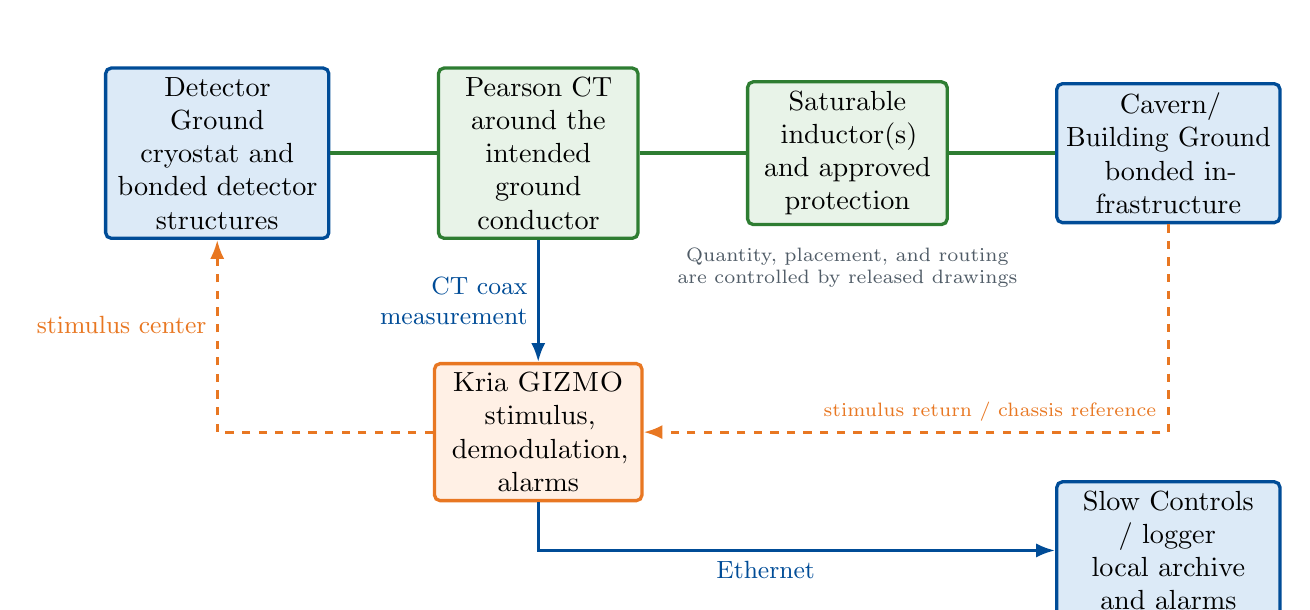
\begin{tikzpicture}[
  >=Latex,
  node distance=1.2cm and 1.35cm,
  box/.style={draw=duneblue,very thick,rounded corners=2pt,fill=dunelightblue,
              align=center,minimum height=1.25cm,text width=2.6cm},
  safety/.style={draw=dunegreen,very thick,rounded corners=2pt,fill=dunelightgreen,
                 align=center,minimum height=1.25cm,text width=2.3cm},
  monitor/.style={draw=duneorange,very thick,rounded corners=2pt,fill=dunelightorange,
                  align=center,minimum height=1.25cm,text width=2.4cm},
  wire/.style={line width=1.5pt,dunegreen},
  signal/.style={line width=1.1pt,duneblue,-{Latex[length=2.4mm]}},
  stimulus/.style={line width=1.1pt,duneorange,dashed,-{Latex[length=2.4mm]}}
]
  \node[box] (det) {Detector Ground\\cryostat and bonded detector structures};
  \node[safety,right=of det] (ct) {Pearson CT\\around the intended ground conductor};
  \node[safety,right=of ct] (si) {Saturable inductor(s)\\and approved protection};
  \node[box,right=of si] (bldg) {Cavern/\\Building Ground\\bonded infrastructure};
  \node[monitor,below=1.55cm of ct] (gizmo) {Kria \GIZMO{}\\stimulus, demodulation, alarms};
  \node[box,below=3.25cm of bldg] (sc) {Slow Controls / logger\\local archive and alarms};

  \draw[wire] (det) -- (ct) -- (si) -- (bldg);
  \draw[signal] (ct) -- node[left,align=right,font=\small]{CT coax\\measurement} (gizmo);
  \draw[stimulus] (gizmo.west) -| node[pos=0.78,left,font=\small]{stimulus center} (det.south);
  \draw[stimulus] (bldg.south) |- node[pos=0.67,above,font=\scriptsize]{stimulus return / chassis reference} (gizmo.east);
  \draw[signal] (gizmo.south) |- node[pos=0.72,below,font=\small]{Ethernet} (sc.west);

  \node[below=0.15cm of si,font=\scriptsize,text=dunegray,align=center]
    {Quantity, placement, and routing\\are controlled by released drawings};
\end{tikzpicture}
\caption{Conceptual measurement topology. The CT must observe the intended return path; any parallel detector-to-infrastructure connection changes the measured signal.}
\label{fig:concept}
\end{figure}

The 2018 Far Site grounding requirements state that the Detector Ground is to remain isolated from other grounding systems except through saturable inductors, require ground-monitoring instrumentation, and call for at least two saturable inductors near the detector isolation transformer with separation greater than six feet. The 2025 Kria ORC package documents a \emph{laboratory} rack containing one MS6984 saturable inductor and one Pearson 2100 CT. The released installation drawing must resolve the final Far Detector quantity and topology; the laboratory ORC drawing must not be copied blindly underground.

\section{Roles and stop-work boundaries}

\begin{tabularx}{\linewidth}{@{}L{0.25\linewidth}Y@{}}
\toprule
Role & Permitted work in this guide \\
\midrule
Authorized electrical worker & Installs and verifies fixed grounding conductors, CT, saturable inductors, protection devices, rack bonds, and approved test fixture under the controlled electrical procedure. \\
\GIZMO{} hardware expert & Verifies chassis, Kria image, analog chain, stimulus amplitude/frequency, calibration, and alarm outputs. \\
Slow Controls / DAQ expert & Configures network, timestamps, one-second fast history, bounded edge retention, off-board replication, archive verification, dashboard, state flags, and stale-data alarm. \\
Construction coordinator & Declares normal/welding/test states, controls the intentional-bond window, records subcontractor activity, and confirms closeout. \\
Operator & Performs the released checklist, watches live status, records events, and stops/escalates when acceptance conditions are not met. \\
\bottomrule
\end{tabularx}

\danger{Stop before energizing or injecting a stimulus if a conductor is unidentified, the CT path is bypassed, the saturable-inductor protection differs from the released drawing, the rack safety bond is missing, the Kria image/configuration is unknown, or no responsible electrical/grounding contact is available.}

\section{Before anyone connects anything}

Complete this section at initial installation and whenever the rack, grounding topology, CT, saturable inductor, firmware, or cryostat connection has changed.

\subsection{Documents and authorization}

\begin{enumerate}
  \item \checkbox\ Confirm the current approved revision of SOP004 GIZMO and the activity-specific hazard analysis.
  \item \checkbox\ Confirm the released Far Detector grounding single-line, cable schedule, CT orientation, saturable-inductor/MOV assembly drawing, and welding plan.
  \item \checkbox\ Confirm the Kria rack ORC is released for the installed location and configuration. DUNE-doc-35392 documents the G271 development rack, not automatically the underground installation.
  \item \checkbox\ Record the equipment IDs: rack, Kria chassis, PDU, CT, saturable inductor(s), AC/DC converter, calibration, software, FPGA image, and configuration hash.
  \item \checkbox\ Name the electrical work lead, \GIZMO{} expert, Slow Controls contact, construction coordinator, and escalation contacts for the shift.
\end{enumerate}

\subsection{Identify the two references}

An authorized electrical worker shall identify and label:

\begin{itemize}
  \item the approved \DetectorGround{} connection/test point;
  \item the approved \InfrastructureGround{} reference/test point;
  \item the intended safety-ground conductor passing through the CT;
  \item the detector side and infrastructure side of the saturable-inductor assembly;
  \item the approved connection point for the stimulus center conductor;
  \item the rack/chassis bonding point used by the stimulus return.
\end{itemize}

\warning{Do not infer ``detector side'' from wire color, physical direction, or an old photograph. Verify the released drawing and labels. The legacy ZedBoard documents refer to transformer secondary X0 and particular busbars; those names may not be the Far Detector Kria installation labels.}

\subsection{Visual and continuity checks}

With the applicable circuits in the safe state and LOTO applied where required:

\begin{enumerate}
  \item \checkbox\ Inspect the rack, CT enclosure, inductor/protection enclosure, connectors, strain relief, and conductor clearances.
  \item \checkbox\ Verify the rack and \GIZMO{} chassis are bonded to \InfrastructureGround{}.
  \item \checkbox\ Verify the intended detector safety-ground path is continuous and matches the approved design.
  \item \checkbox\ Verify the CT surrounds only the intended conductor(s), is mechanically secure, and is not bypassed by an unmonitored parallel conductor.
  \item \checkbox\ Verify no temporary welding lead, shield, pipe bond, test jumper, construction cable, or tool bridges Detector Ground and Cavern/Building Ground.
  \item \checkbox\ Verify the alarm beacon is visible and the audible device is appropriate for the work area.
\end{enumerate}

\section{Connection sequence}

This sequence describes the signal and rack interfaces. Fixed grounding work remains the responsibility of the authorized electrical worker and the controlled installation procedure.

\subsection{Make connections with the rack de-energized}

\begin{enumerate}
  \item \textbf{Safety-ground assembly.} The authorized electrical worker installs or verifies the approved Detector Ground--CT--saturable-inductor/protection--Cavern/Building Ground path. Do not open this path as part of routine \GIZMO{} work.

  \item \textbf{CT signal.} Connect the approved coaxial cable from the Pearson CT output to the \GIZMO{} connector designated \textsc{CT INPUT}. Verify both endpoint labels and cable ID.

  \item \textbf{Stimulus.} Connect the stimulus output using the approved custom cable:
  \begin{itemize}
    \item the center conductor goes to the designated Detector Ground-side injection point;
    \item the outer conductor/return is bonded to the designated rack or Cavern/Building Ground point.
  \end{itemize}
  Do not improvise this cable or move the injection point without repeating characterization.

  \item \textbf{Alarm outputs.} Connect the warning beacon and audible alarm to the labeled \GIZMO{} outputs. Do not use an alarm-power connector as a general auxiliary supply.

  \item \textbf{Network.} Connect the Kria \GIZMO{} Ethernet port to the assigned detector controls network switch port. Connect the Raritan PDU management port separately if required by the rack drawing.

  \item \textbf{DC power.} Connect the approved NRTL-listed AC/DC converter to the Kria chassis. DUNE-doc-35392 identifies a $12\,\mathrm{VDC}$, $5\,\mathrm{A}$ converter for the development rack. Verify the installed chassis label before connection.

  \item \textbf{PDU input.} Connect the Raritan PDU only to the approved branch circuit and adapter specified by the installed rack ORC. Check protective-earth continuity before energizing.
\end{enumerate}

\danger{Never perform make-before-break or bypass work on the CT/safety-ground conductor from this guide. The old setup package references a separate CT bypass procedure. That operation requires its own released procedure, tools, hazard controls, and authorized electrical worker.}

\subsection{Independent connection verification}

Before power-up, a second qualified person should perform a point-to-point check against the released drawing. Read each cable label aloud and record initials for:

\begin{center}
\begin{tabularx}{0.94\linewidth}{@{}Y L{0.19\linewidth} L{0.19\linewidth}@{}}
\toprule
Connection & Installed by & Verified by \\
\midrule
CT output $\rightarrow$ \GIZMO{} CT input & & \\
Stimulus center $\rightarrow$ approved Detector Ground-side point & & \\
Stimulus return/chassis $\rightarrow$ approved Cavern/Building Ground & & \\
Beacon and audible alarm outputs & & \\
Kria and PDU network ports & & \\
$12\,\mathrm{VDC}$ supply and PDU branch circuit & & \\
Safety path and CT routing match released drawing & & \\
\bottomrule
\end{tabularx}
\end{center}

\section{Step-by-step power-up}

\subsection{Pre-power state}

\begin{enumerate}
  \item \checkbox\ Confirm work state is \texttt{COMMISSIONING} or \texttt{NORMAL}; no undeclared welding activity is in progress.
  \item \checkbox\ Confirm all connection-verification rows above are signed.
  \item \checkbox\ Confirm the approved logging and archive plan is available, the Kria has sufficient storage headroom, and every required off-board replica is provisioned for post-boot verification.
  \item \checkbox\ Confirm the approved Kria software/FPGA/configuration identifiers are available. If any identifier is unknown, record it as unknown and do not claim the system is commissioned.
  \item \checkbox\ Confirm the selected excitation is disabled until the electrical lead authorizes injection.
\end{enumerate}

\subsection{Energize and verify}

\begin{enumerate}
  \item Energize the rack PDU from the approved branch circuit. Verify normal PDU status and protective-earth indication.
  \item Energize the Kria \GIZMO{} $12\,\mathrm{VDC}$ supply. Check for normal front-panel power indicators, abnormal sound, odor, heat, or smoke. De-energize immediately if any abnormal condition appears.
  \item Wait for the approved Kria boot interval. Confirm \texttt{gizmo.target} and the required component services are healthy through the approved operational workflow; record the installed runtime and model versions.
  \item Verify OPC~UA reachability from the assigned Slow Controls host, resolve \texttt{urn:fnal:gizmo} at connection time, and validate device identity. Use the registered hostname, address, certificate, and trust policy from site configuration; do not use historic ZedBoard connection data from old documents.
  \item Verify the system clock and data timestamp are UTC and advancing. The legacy display required the measurement time to remain within 10 seconds of the system time; the Kria acceptance criterion is \TBD.
  \item Start the approved acquisition target and confirm the configured excitation waveform, frequency, amplitude limit, and calibration ID before enabling stimulus. Public service names and commands are documented in the maintained Kria runtime; their use still requires the site-approved procedure.
  \item With authorization from the electrical lead, enable the configured stimulus only after its waveform, frequency, and amplitude have been approved for the installed topology. Record the actual settings; do not substitute a legacy nominal value.
  \item Confirm the local historian records one fast snapshot per second, sequence numbers advance, timestamps are monotonic, platform snapshots arrive every ten seconds, and no parse/quality flags are set.
  \item Confirm a plausible stable reading against the most recent commissioned baseline. Do not use a ProtoDUNE, LArTF, MINOS, or laboratory resistance value as the Far Detector baseline.
  \item Verify the dashboard shows impedance, threshold, data age, hardware state, work state, and alarm state. Confirm the SQLite edge store is advancing and every configured replica cursor is healthy.
\end{enumerate}

\good{The system is ready for routine monitoring only when the reading is stable around the commissioned baseline, the alarm threshold and calibration ID are correct, data age is within its limit, local storage is active, and the work state is explicitly recorded.}

\subsection{What remains site-controlled}

The public Kria runtime defines the component services, canonical OPC~UA
namespace, typed monitoring values, bounded configuration writes, operations,
historian, and dashboard. It intentionally does not publish production
endpoints, credentials, certificate material, target images, calibration
state, network configuration, or authorization policy. The controlled
revision of this guide must identify the approved runtime/configuration,
endpoint, trust and role policy, exact field commands, rollback, and recovery
steps. Legacy commands such as \texttt{./GIZMO.elf}, \texttt{RUN},
\texttt{load\_f}, and \texttt{set\_th} are not Kria commands.

\section{Commissioning and baseline}

Commissioning establishes what ``normal'' means for the actual cryostat, grounding conductors, saturable inductors, CT, stimulus cable, and installed firmware. A threshold without a site-specific characterization is not defensible.

\subsection{Characterization prerequisites}

The legacy characterization procedure requires equipment powered from the detector isolation transformer to be powered down, the transformer primary locked out/tagged out, and detector-ground connections controlled before a decade box is inserted. Apply the current approved equivalent; do not reproduce that test casually during construction.

Use only an approved resistive/capacitive test fixture. The test plan should obtain:

\begin{itemize}
  \item open/reference response and noise distribution;
  \item response to known resistances spanning normal isolation through alarm conditions;
  \item response to known capacitances representative of the installed detector;
  \item frequency response over the approved scan range;
  \item response with representative construction equipment on and off;
  \item end-to-end verification of beacon, audible alarm, Slow Controls alarm, and logging flags.
\end{itemize}

\subsection{Frequency selection}

Select the operating frequency from measured data, not tradition alone. The chosen frequency should:

\begin{enumerate}
  \item avoid resonances of the installed saturable-inductor and detector-capacitance network;
  \item avoid strong coherent facility or switching-noise lines;
  \item provide a large and monotonic separation between the open/normal state and known resistive shorts;
  \item provide stable I/Q demodulation and acceptable variance over representative work conditions;
  \item remain within the approved stimulus-current and touch/noise limits.
\end{enumerate}

Record the sweep, fit, chosen frequency, waveform, amplitude, uncertainty, calibration file/hash, and approver. Changing frequency, amplitude, CT, stimulus routing, saturable inductor, or major cryostat bonding requires review and normally re-characterization.

\subsection{Threshold selection}

The threshold is a site-specific engineering decision. A useful proposed rule is to place it far enough from the normal distribution to avoid nuisance alarms, while guaranteeing detection of the maximum short resistance that must be found. Document both margins using the characterization data. Do not copy the legacy $100\,\Omega$ example or historic $5$--$6\,\Omega$ direct-short reading into the Far Detector configuration without validation.

\section{Routine live monitoring}

\subsection{At the beginning of a shift}

\begin{enumerate}
  \item Confirm the work-state selector is correct: \texttt{NORMAL}, \texttt{WELDING}, \texttt{TEST}, \texttt{MAINTENANCE}, or \texttt{UNKNOWN}.
  \item Confirm data age is below the approved stale limit and the last record time is current UTC.
  \item Confirm measured impedance is above the approved alarm threshold and within the baseline band.
  \item Confirm frequency, amplitude, calibration ID, firmware/configuration ID, and threshold match the shift reference.
  \item Review the previous 12 hours for steps, drift, gaps, or unclosed welding windows.
  \item Confirm local historian, free-space guard, replica cursor, and archive status. Record the check in the shift log or Procore summary.
\end{enumerate}

\subsection{Minimum live display}

The operator should see, on one screen:

\begin{itemize}
  \item current impedance/resistance and threshold, in ohms;
  \item a time trend with at least the previous 12 hours;
  \item I, Q, and magnitude or equivalent Kria diagnostics;
  \item data age and sample quality;
  \item excitation frequency and enabled state;
  \item hardware/configuration/calibration IDs;
  \item current construction work state and active welding permit/window;
  \item local historian, replica, archive, and network health;
  \item alarm status and acknowledgement history.
\end{itemize}

\subsection{Logging format and retention}

The implemented Kria historian uses SQLite schema version~2. Do not use a
Procore spreadsheet as the raw data store and do not copy the live SQLite file
while its WAL writer is active. Create an immutable archive with the SQLite
online-backup API or a checkpointed export, then record its checksum, schema
version, runtime version, model digest, and capture-path digest in the
controlled archive manifest.

\begin{tabularx}{\linewidth}{@{}L{0.25\linewidth}L{0.2\linewidth}Y@{}}
\toprule
Record class & Implemented cadence / retention & Purpose \\
\midrule
Fast snapshot & 1 second / 14 days on Kria & Measurement, authoritative alarm, lock-in values, phase, thermal values, uptime, and sequence. \\
Platform snapshot & 10 seconds / 30 days on Kria & Chartable operating-system, storage, process, filesystem, and network counters. \\
Minute rollup & 1 minute / 365 days on Kria & First, last, minimum, maximum, mean, count, and worst OPC~UA status. \\
Transition event & on change / 1825 days on Kria & Alarm, quality, clock, boot, network, service, and historian state changes. \\
\bottomrule
\end{tabularx}

Every stored scalar retains its OPC~UA value, StatusCode, and source timestamp;
the row also records historian receive time and, for fast data, sequence and
stream epoch. Raw SDR/ADC frames are excluded. The measured planning rate is
approximately 1.48~GB per continuously operating month. The bounded Kria
policy occupies about 1.26~GB in replay; a permanent off-board replica may
disable age-based pruning while retaining the free-space guard and independent
backup requirements.

Replication is cursor-based, bounded, transactional, and idempotent. It
transfers inserts and updated rollups, never deletion. The board-local store
is the authoritative edge buffer; each off-board replica and the site Ignition
historian are independent downstream records with their own retention and
restore acceptance.

Procore should contain human summaries and controlled events:

\begin{itemize}
  \item automatically generated 6-, 12-, or 24-hour plots and statistics;
  \item shift start/end checks;
  \item welding-window start/end and permit/work-package reference;
  \item alarm events, acknowledgements, investigation, and disposition;
  \item links to the immutable archive, checksum, configuration, and calibration.
\end{itemize}

\section{Welding and other planned ground shorts}

Welding may intentionally connect Detector Ground to Cavern/Building Ground through the welding equipment or a temporary bonding arrangement. During that interval, a low \GIZMO{} reading is expected, but it also masks any second accidental short. The work window must be controlled and time-correlated with the data.

\subsection{Before the welding window}

\begin{enumerate}
  \item The construction coordinator confirms the approved welding procedure, work package, location, subcontractor supervisor, expected grounding/bonding arrangement, and start/end authorization.
  \item The electrical/grounding lead confirms that the welding return and temporary bonds match the approved plan. \GIZMO{} does not authorize or validate welding-current routing.
  \item The operator verifies at least five minutes of stable pre-work baseline with no active alarm or data-quality issue. Five minutes is a proposed operational value and must be approved in SOP004.
  \item Record a \texttt{WELDING\_PREP} event with UTC time, work-package ID, location, company, supervisor, and expected duration.
  \item Confirm continuous one-second fast-history capture and a healthy edge buffer. Do not stop acquisition because a short is expected.
  \item If audible/visual alarms must be inhibited to conduct the work, use only the approved software alarm-management method. Preserve raw data and an unmistakable \texttt{ALARM\_INHIBITED} flag. Do not disconnect the CT, stimulus, safety-ground path, or monitor to silence an alarm.
\end{enumerate}

\subsection{When the intentional bond is made}

\begin{enumerate}
  \item Record \texttt{WELDING\_ACTIVE} at the actual time the bond/return becomes effective.
  \item Confirm \GIZMO{} sees the expected transition. If no change is observed when the approved topology predicts one, stop and ask the grounding/\GIZMO{} expert to verify the measurement path.
  \item Keep the dashboard visible and monitor data age, hardware health, and logging continuity. Impedance alone is not a valid isolation indicator while the intentional short exists.
  \item Record any additional temporary bonds, cable changes, moves, pauses, or work-area changes as timestamped events.
  \item Treat a loss of \GIZMO{} data as loss of construction monitoring. Pause ground-affecting work unless the approved work plan explicitly defines an alternative.
\end{enumerate}

\subsection{Close the welding window}

\begin{enumerate}
  \item The subcontractor confirms welding has stopped and all temporary leads/bonds identified in the work plan have been removed or placed in their specified final state.
  \item Record \texttt{WELDING\_BOND\_REMOVED} at the actual removal time.
  \item Verify the impedance returns toward the pre-work baseline and the normal alarm state restores. The legacy system recovered within approximately three seconds after removing a test short; use the measured Kria recovery time and approved acceptance window.
  \item Require a stable post-work interval. A proposed quantitative criterion is: no bad-quality flags and all samples remain within the larger of the approved absolute tolerance or $3\sigma$ of the pre-work baseline for at least 60 seconds. The grounding group must approve the final criterion.
  \item If the reading does not recover, keep the work area controlled. Do not begin by removing the safety ground. Inspect the newly installed work, temporary leads, shields, piping, scaffolding, tools, and recent cable connections using the approved fault-isolation plan.
  \item Record \texttt{WELDING\_CLOSED} only after the electrical/grounding lead and construction coordinator accept the post-work state. Attach the before/after plot to the shift or Procore record.
\end{enumerate}

\danger{An intentional welding short is not a nuisance alarm to be ignored. It is a declared alternate system state. If the work state is unknown, the welding window has expired, or the physical bond configuration does not match the approved plan, treat the low reading as an unexpected ground fault.}

\section{Alarm and fault response}

\begin{longtable}{@{}L{0.24\linewidth}L{0.27\linewidth}L{0.43\linewidth}@{}}
\toprule
Observation & Meaning & Immediate operator response \\
\midrule
\endhead
Impedance below threshold during \texttt{NORMAL} & Possible new conductive path between ground references & Stop new ground-affecting work; record UTC time; notify construction coordinator and grounding expert; preserve data; inspect recent changes under the approved fault plan. Never lift the safety ground. \\
\addlinespace
Impedance below threshold during declared \texttt{WELDING} & Expected intentional bond, but additional shorts are masked & Verify active work package, location, and time window. Continue data/health monitoring. If the declared state is wrong or expired, handle as an unexpected fault. \\
\addlinespace
Sudden step that remains above threshold & Topology or capacitive coupling may have changed & Record event, identify simultaneous work, compare I/Q and magnitude, and ask the grounding expert whether a new baseline/characterization is required. \\
\addlinespace
Stale timestamp, missing samples, or sequence gaps & Monitoring coverage is lost or degraded & Raise a distinct stale-data alarm. Pause ground-affecting work unless the approved procedure provides an alternative monitor. Recover the logger without erasing the local file. \\
\addlinespace
Implausible value, clipping, I/Q discontinuity, or frequency mismatch & Analog chain, CT, stimulus, configuration, or calibration problem & Mark data invalid; do not reinterpret it as good isolation. Check configuration ID and hardware status; escalate to the \GIZMO{} expert. \\
\addlinespace
Alarm does not activate during an authorized test & End-to-end protection/notification failure & Do not release to routine monitoring. Verify threshold, test fixture, beacon, audible output, Slow Controls path, and CT/stimulus topology. \\
\bottomrule
\end{longtable}

\subsection{Fault-isolation principle}

Look first at what changed immediately before the transition. Use construction records to divide the search by area or work package. Disconnect or isolate candidate paths only under the controlling procedure and with the responsible system owner. Never use \GIZMO{} as permission to disconnect protective grounding or defeat electrical safety.

\section{Normal shutdown and maintenance}

\begin{enumerate}
  \item Record the reason, UTC time, current work state, impedance, threshold, configuration ID, and last healthy sample.
  \item Close or pause ground-affecting construction work unless the approved plan provides another active monitor.
  \item Verify the last historian write and every required replica cursor. If an archive is required, create a consistent online backup or checkpointed export, calculate its checksum, and record the storage reference.
  \item Disable the excitation using the approved Kria control: \TBD. Confirm the status reports stimulus off.
  \item Stop the acquisition service using the approved Kria method: \TBD.
  \item De-energize the Kria chassis and rack PDU only when authorized by the rack procedure.
  \item Disconnect signal, network, or DC cables only after power is off and the work is released.
  \item Leave the permanent safety-ground and saturable-inductor path in its approved state. Any work on it requires the separate electrical procedure.
\end{enumerate}

\section{Legacy ZedBoard reference}

This section helps experts interpret the old unit and historical data. It is not the Kria operating procedure.

\subsection{Legacy hardware and operation}

The old \GIZMO{} uses a ZedBoard with a Xilinx Zynq XC7Z020, a 16-bit DAC, and a 12-bit ADC operating at approximately $1\,\mathrm{MS/s}$. Firmware provides deterministic stimulus/acquisition timing. Linux software demodulates the digitized waveform to I and Q, applies low-pass filtering, and derives magnitude and a calibrated resistance estimate.

The 2022 engineering note specifies an approximately $22\,\mathrm{mA}$ peak-to-peak, $1.4\,\mathrm{kHz}$ sine stimulus; the older 2017 note specifies approximately $100\,\mathrm{mA}$ peak-to-peak. This is a hardware/software revision difference and another reason to record configuration rather than assume an amplitude.

Historical shell output has the form:

\begin{verbatim}
RES=154.8  TH=100 ( mag=268.640, I=265.217, Q=-42.746 )
\end{verbatim}

The public LArTF client polls the shell every two seconds and writes \texttt{RES}, \texttt{TH}, \texttt{mag}, \texttt{I}, and \texttt{Q} to InfluxDB. Its hostname, account, host-key policy, paths, and authentication behavior are historical examples and must not be reused as a production security design.

The planned legacy OPC~UA server is expected to publish the common
\texttt{urn:fnal:gizmo} contract and explicit non-good quality for unsupported
or stale values. This guide assumes that work proceeds, but the server remains
a commissioning dependency: Ignition history and alarms shall not be enabled
until identity, coherent-cycle, display-comparison, restart, network-loss, and
read-only-boundary tests pass.

\subsection{Legacy-only checks}

For a correctly configured legacy unit:

\begin{itemize}
  \item power-up normally starts monitoring automatically, but different document revisions disagree on whether the last threshold is retained or a $500\,\Omega$ alarm threshold is loaded after a power cycle;
  \item the front panel displays measured resistance, threshold, system time, and last-measurement time;
  \item system and measurement times should differ by no more than 10 seconds;
  \item \texttt{RUN} loads the $1.4\,\mathrm{kHz}$ waveform automatically;
  \item changing \texttt{threshold.txt}, using \texttt{set\_th}, running \texttt{CAL}, changing waveform/amplitude, or manipulating relays is expert work tied to the installed image.
\end{itemize}

\section{Kria commissioning record and open items}

The following fields must be completed before this draft can become a field procedure.

\begin{longtable}{@{}L{0.38\linewidth}L{0.52\linewidth}@{}}
\toprule
Controlled item & Approved value / reference \\
\midrule
\endhead
Underground rack ID and released ORC & \TBD \\
Far Detector grounding single-line and cable schedule & \TBD \\
Saturable-inductor quantity, IDs, protection, and placement & \TBD \\
Pearson CT ID, orientation, cable ID, and transfer factor & \TBD \\
Detector-side stimulus connection point & \TBD \\
Cavern/Building Ground stimulus return point & \TBD \\
Kria hostname, OPC~UA endpoint, certificate/trust policy, and network owner & \TBD \\
Kria OS, FPGA image, application, and configuration IDs & \TBD \\
Approved runtime version; startup, enable, disable, restart, and recovery commands & \TBD \\
Boot time, update cadence, stale-data limit, and recovery time & \TBD \\
Excitation waveform, frequency, amplitude, and tolerance & \TBD \\
Calibration file/hash, validity range, uncertainty, and owner & \TBD \\
Normal baseline band and alarm threshold & \TBD \\
Authorized alarm-test fixture and procedure & \TBD \\
Slow Controls endpoint, roles, selected fields, status bits, and alarms & \TBD \\
Historian schema~2 archive, local retention, checksum, and restore record & \TBD \\
Off-board replica/archive destination, retention, and owner & \TBD \\
Welding-state interface and authorized alarm-inhibit method & \TBD \\
Shift, electrical, grounding, Slow Controls, and emergency contacts & \TBD \\
\bottomrule
\end{longtable}

\section{Shift record template}

\begin{tabularx}{\linewidth}{@{}L{0.30\linewidth}Y@{}}
\toprule
Date / shift / operator & \\
Rack / chassis / configuration ID & \\
Calibration ID / threshold & \\
Excitation waveform / frequency / amplitude & \\
Baseline at shift start & \\
Data age / historian / replica / archive status & \\
Active work state / work package & \\
Welding windows and subcontractor lead & \\
Alarms, steps, gaps, or interventions & \\
Baseline at shift end & \\
Archive reference and checksum & \\
Summary plot / Procore record & \\
Open issues and handoff & \\
\bottomrule
\end{tabularx}

\section{Source documents}

\begin{enumerate}
  \item DUNE-doc-35392-v2, \emph{ORC Documents for DUNE Impedance Monitor Rack in FNAL HEERC G271}. Current Kria rack hardware basis; laboratory/development configuration.\\
  \url{https://docs.dunescience.org/cgi-bin/private/ShowDocument?docid=35392}

  \item DUNE-doc-1805-v12, \emph{GIZMO: Ground Current Impedance MOnitor}. Legacy engineering note, operations, setup instructions, diagrams, and schematics.\\
  \url{https://docs.dunescience.org/cgi-bin/private/ShowDocument?docid=1805}

  \item DUNE-doc-25365-v1, \emph{LArTF Impedance Monitor System for 2x2}. 2022 engineering note, characterization, and operating tips.\\
  \url{https://docs.dunescience.org/cgi-bin/private/ShowDocument?docid=25365}

  \item DUNE-doc-27482-v2, \emph{MINOS Impedance Monitor System}. Legacy SD-card, chassis, calibration, PMOD, and testing material.\\
  \url{https://docs.dunescience.org/cgi-bin/private/ShowDocument?docid=27482}

  \item DUNE-doc-285-v11, \emph{DUNE Grounding Plan}; file \emph{LBNF/DUNE Far Site Detector Grounding System Requirements}, April 8, 2018.\\
  \url{https://docs.dunescience.org/cgi-bin/private/ShowDocument?docid=285}

  \item D. Subedi, \emph{Ground Impedance Monitor Technical Report}, 2021. ZedBoard architecture and Far Detector frequency study.\\
  \url{https://dsubedi.info/data/I1/FNAL_2021_GIZMo_paper.pdf}

  \item V. Cerrone, \emph{DUNE ND-LAr 2x2 Demonstrator Tests}, 2022. Legacy SSH, InfluxDB, and Grafana readout implementation.\\
  \href{https://indico.fnal.gov/event/56266/contributions/251018/attachments/160238/211768/Cerrone_report.pdf}{Fermilab Indico report attachment}

  \item Public legacy client source, \texttt{gizmo\_control}.\\
  \url{https://github.com/vanessacerrone/gizmo_control}

  \item Public GIZMo Kria runtime, OPC~UA contract, historian, and dashboard
  documentation.\\
  \url{https://github.com/marroyav/GIZMo}

  \item Public GIZMo Slow Controls ICD and dual-platform DCS intake package.\\
  \url{https://github.com/marroyav/gizmo-icd}

  \item Public GIZMo historian archive schema and verification tools.\\
  \url{https://github.com/marroyav/gizmo-data-archive}

  \item Public GIZMo Ignition project and history-migration tooling.\\
  \url{https://github.com/marroyav/gizmo-ignition}
\end{enumerate}

\warning{Several source documents describe prototypes or installations other than the DUNE Far Detector. Their values are clearly labeled as legacy or proposed in this guide. The current released drawings, Kria software manual, site characterization, and approved work controls take precedence.}

\vfill
\begin{center}
\small\textcolor{dunegray}{End of integration and commissioning draft}
\end{center}

\end{document}
